\section{Kernel}
% ----------
\subsection{Compilation}
\begin{itemize}
    \item Configuration : \verb!make linux-menuconfig!
    \item Compilation : \verb!make linux-rebuild!
\end{itemize}
% ----------
\subsubsection{Amélioration}
Option \verb!-fstack-protector-all!: (idem u-boot) ajout d'un canary.

Option \verb!Randomize_va_space!: permet de placer les éléments à des emplacements mémoire aléatoires (pour éviter d'en cibler un facilement).

Optimisation du kernel pour la place OU pour les performances.

Strip l'assembleur: suppression des symboles non nécessaires (commentaire de debug), pour éviter reverse-engineering du code. 

Restriction de l'accès au syslog (system logs).

Mise à 0 lors de l'allocation dynamique sur le tas ou la pile: permet d'éviter à l'attaquant de récupérer des données ou du code.
% ----------
\subsection{Busybox}
Busybox: logiciel qui regroupe plusieurs outils/fonctions de base (\verb+ls+, \verb+mv+, \verb+rm+, \verb+cat+, etc.). En mettant toutes ces commandes dans un seul programme, on réduit énormément les redondances et par conséquent la taille de l'éxécutable.
\begin{itemize}
    \item Configuration: \verb!make busybox-menuconfig!
    \item Compilation: \verb!make busybox-rebuild!
\end{itemize}

% ----------
\subsection{Réseau}
Si le système n'est pas un routeur, on peut choisir de désactiver le routage et le \verb!rp_filter! doit être activé sur toutes les interfaces.
% ----------
\subsection{Attaques}
\begin{figure}[H]
    \centering
    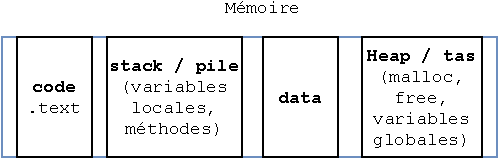
\includegraphics[width=0.6\columnwidth]{kernel.pdf}
\end{figure}
\paragraph{Éxecution sur le stack (buffer overflow)} : Insertion de code exécutable dans le stack. Attaque plus possible à présent car le stack est non-exécutable.
\paragraph{ret2libc} : Permet de bypasser la non-éxécution du stack. Consiste à éxécuter du code dans une librairie comme libc.
\paragraph{ROP (Return-Oriented Programming)} : Éxécution de code malveillant à l'intérieur du programme lui-même. Exploitation des vulnérabilités de sécurité dans le code pour exécuter du code arbitraire en combinant des fragments de code valides déjà présents dans le processus. Au lieu d'injecter du code malveillant dans le processus, on utilise des instructions de retour pour construire une chaîne d'instructions spécifiques.
\subsection{Protections}
\label{sec_protections}
\paragraph{ASLR (Address Space Layout Randomization)} : déplacement aléatoire des adresses mémoires (du stack et du heap) à chaque redémarrage du système, il n'est ainsi plus possible de prédire la localisation des instructions placées en mémoire p.ex. avec un buffer overflow. $\Rightarrow$ évite les attaques \verb+ret2libc+.
\paragraph{PIE (Position Independent Executable)} : Rend tout le code exécutable aléatoirement positionné, similaire à ASLR mais agit sur tout l'exécutable.
\paragraph{Canary} : Variable qui permet de détecter un dépassement dans le stack. Elle peut être de valeur fixe, ou générée aléatoirement.